\documentclass{article}
\usepackage{rotating}
\usepackage{hyperref}
\usepackage[margin=1in]{geometry}
\title{ FMC Delay 1ns 4cha (Fine Delay) \\ \large{Long term test report}}

\author{Tomasz Wlostowski, CERN BE-CO-HT}
\date{September 2013, git version: \ttfamily{ddbf6ec}}
\begin{document}
   \maketitle
\section{Introduction}
This report provides a summary of tests performed on a specimen of the Fine Delay (FmcDelay1ns4cha, further abbreviated as FD) card \cite{homepage}.
The purpose of these tests was to:
\begin{itemize}
\item Check the stability of the card's operation over a long period of time.
\item Gather statistics of trigger-to-output delay.
\end{itemize}

The report does not cover all possible delay values, as it would be impractical due to very wide delay range (up to 120 seconds) supported by the FD. The VHDL was designed and verified on simulation in such a way that passing the long term test at a single delay setting automatically proves stability for other delay values (as the test assumes that trigger pulses are uncorrelated with the card's reference clock).

\section{Measurements}
\subsection{Setup}
The measurement system used is depicted in Figure \ref{fig:meas_system}. It consists of:


\begin{itemize}
\item Pulse source: a HP 33250A waveform generator (S/N: MY40001267).
\item Time interval meter: Pendulum CNT-91 \cite{cnt91} (S/N: 205575), measuring the trigger-to-output delay of the FD mezzanine. Only 1 output of the FD was used, as other outputs have an identical structure (and we don't have enough CNT-91's...).
\item FD mezzanine (version V5-2 \cite{edms}, S/N: CR000010) under test with a SVEC carrier \cite{svec}, hosted in a VME64x crate with a MEN A20 controller.
\item PC running Linux for data logging and controlling the CNT-91 TDC.
\item Software for the MEN A20 and the PC for data logging (C program and some Python scripts). Temperature and timestamp data were sent from the VME crate to the PC via a TCP connection.
\end{itemize}

\begin{figure}[htb]
\centering
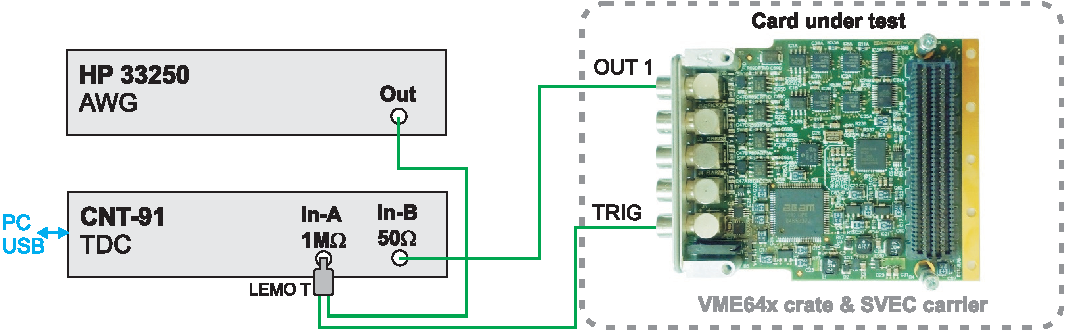
\includegraphics[width=16cm]{drawings/connection_diagram}
\caption{Long term measurement setup.}
\label{fig:meas_system}
\end{figure}

The card's trigger input was fed with 2 microsecond-wide pulses of 3 V amplitude and a 100 Hz rate, with a 50 $\Omega$ input termination. The card was configured to introduce a 700 ns delay. A low delay value was chosen to eliminate the drift of the local oscillator from the results (which in the long term could hide random/spurious artifacts such as incorrect FD's TDC timestamps).

For each trigger pulse, the following parameters were recorded:
\begin{itemize}
\item Trigger-to-output delay, measured with the CNT-91.
\item Board temperature, measured using the integrated temperature sensor.
\item TDC timestamp, read by the driver.
\end{itemize}

\subsection{Results}

The tests consist of two continuous runs, one of 14 days and another of 34.5 days, that is ~48.5 days in total. 
There was a short gap between the two series caused by reconfiguration of the CERN network.

Table \ref{tbl:summary} summarizes all the samples gathered. The uncorrected jitter value is based on raw delay 
measurements taken from the CNT-91. The corrected one compensates for the the jitter of the 
CNT-91 (done by subtracting squared standard deviations assuming that both CNT-91 and FD jitter is of Gaussian shape and independent).

\begin{table}[h]
  \centering
\caption{Long term delay statistics.}
\vskip 2mm
\begin{tabular}{ l | l }
\bfseries{Parameter} & \bfseries{Value} \\
\hline
Total samples & 419,157,455\\
Cabling delay & 12.7 ns\\
Average delay & 699.94 ns\\
Maximum delay & 700.54 ns\\
Minimum delay & 699.5 ns\\
Worst case error & 0.59 ns\\
Uncorrected rms jitter & 72 ps\\
CNT-91 rms jitter & 31 ps\\
Corrected rms jitter & 65 ps\\
CNT-91 maximium delay & -0.12 ns\\
CNT-91 minimium delay & 0.12 ns\\
Minimum temperature & 65 degrees C\\
Maximum temperature & 68 degrees C \\
\end{tabular}

\label{tbl:summary}
\end{table}

Short-term stability was characterized by picking a 1-minute long averaging window. The results are presented in Table \ref{tbl:summary_notemp}.

\begin{table}[h]
  \centering
\caption{Short term delay statistics.}
\vskip 2mm
\begin{tabular}{ l | l }
\bfseries{Parameter} & \bfseries{Value} \\
\hline
Number of samples & 6000\\
Average delay & 699.93 ns\\
Maximum delay & 700.28 ns\\
Minimum delay & 699.62 ns\\
Worst case error (wrs to the average delay) & 300 ps\\
Typical ACAM rms jiitter & 41 ps\\
Delay line rms jitter & 10 ps\\
Theoretical rms jitter & 42 ps\\
Measured rms jitter & 57 ps\\
\end{tabular}

\label{tbl:summary_notemp}
\end{table}

The plot in Figure \ref{fig:plot_average} visualizes the short term average, minimum and maximum delay values. 

\begin{figure}[htb]
\centering
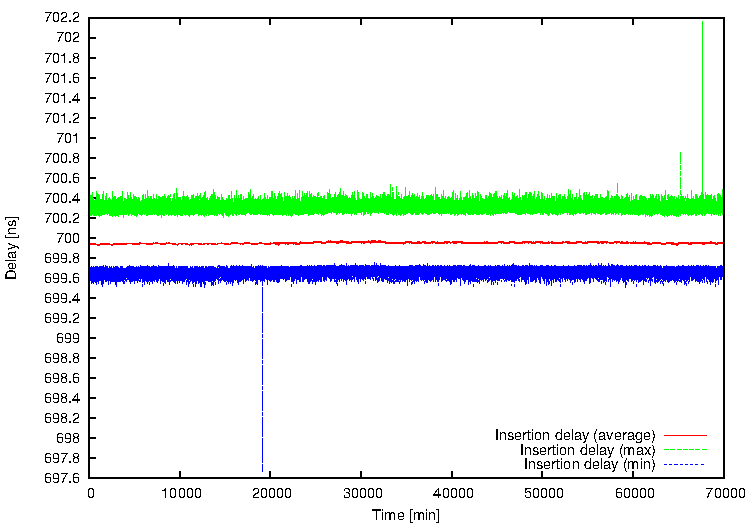
\includegraphics[width=13cm]{drawings/plot_average}
\caption{Average, minimum and maximum trigger-to-output delay (sliding average with a 1-minute window).}
\label{fig:plot_average}
\end{figure}

During the entire test, 3 events outside the specified range were discovered:
\begin{itemize}
\item sample 114714751: 697.67 ns (-2.33 ns error)
\item sample 391199777: 700.86 ns (0.86 ns error)
\item sample 406143035: 702.16 ns (2.16 ns error)
\end{itemize}

We attribute these errors to the ACAM TDC \cite{acam}, as they exist both in the timestamps read out by the driver (the input signal is periodic) and in the measured delays. Similar events have been observed
for the \emph{FmcTdc} card \cite{fmctdc} and in older versions of the FD firmware, where the TDC works in a different mode (respectively, I- and R-modes).

To our knowledge, this test is the first public, long term stability test of the ACAM TDC-GPX chip. Given the size of the statistics data, 3 out of 420 million events are extremely rare (below 7 sigma threshold) and do not exceed
2.5 ns (the typical applications advertised for this chip, such as PET tomography, spectroscopy of laser rangefinders are likely not concerned by such a low error rate).

The plot in Figure \ref{fig:jitter_histogram} shows the histogram of the jitter in the measured delay values. It resembles a gaussian shape. Note that certain bins are empty due to the discrete nature of both the FD and the CNT-91.

\begin{figure}[htb]
\centering
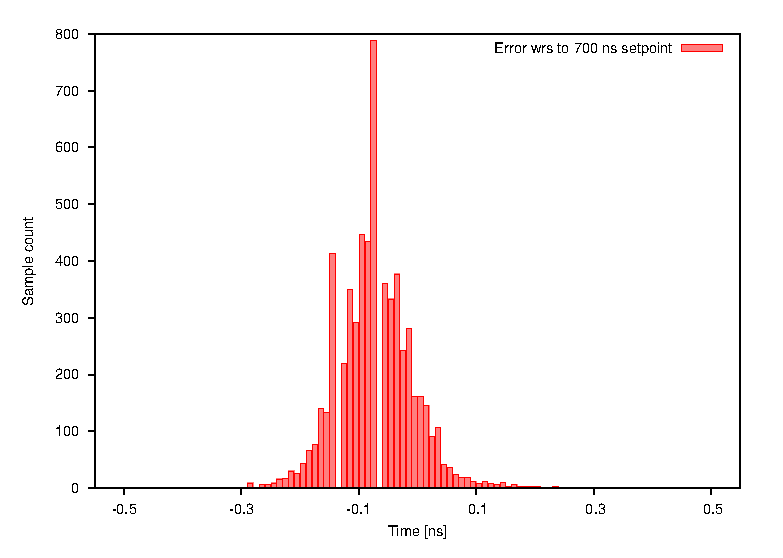
\includegraphics[width=13cm]{drawings/jitter_histogram}
\caption{Histogram of trigger-to-output jitter.}
\label{fig:jitter_histogram}
\end{figure}

\section{Summary}

\textbf{Final results have confirmed long term stability and compliance of the card with the specification}:

\begin{itemize}
\item Absolute delay accuracy is better than 1 ns,
\item Input-to-output rms jitter (standard deviation) is better than 100 ps. 
\end{itemize}

Further testing with a climatic chamber could be performed to determine the effects of temperature on the jitter and accuracy, and allow the software to compensate for them, if needed.

\begin{thebibliography}{9}

\bibitem{edms}
  Official schematics and PCB design (CERN EDMS), \url{https://edms.cern.ch/nav/EDA-02267-V5-2}
\bibitem{homepage}
  Fine Delay hardware homepage and Wiki, \url{http://www.ohwr.org/projects/fmc-delay-1ns-8cha}
\bibitem{manual}
  Official user's manual, \url{http://www.ohwr.org/documents/179}
\bibitem{svec}
  SVEC FMC Carrier Project, \url{http://ohwr.org/projects/svec}
\bibitem{cnt91}
  Pendulum CNT-91 TDC/Frequency meter, \href{http://www.spectracomcorp.com/ProductsServices/TestandMeasurement/FrequencyAnalyzersCounters/CNT9191RTimerCounterAnalyzerCalibrator/tabid/1283/Default.aspx}{manufacturer's website}
\bibitem{acam}
  ACAM TDC-GPX TDC chip, \url{http://www.acam.de/products/time-to-digital-converter/tdc-gpx}
\bibitem{fmctdc}
  FmcTdc1ns5cha project, \url{http://www.ohwr.org/projects/fmc-tdc}

\end{thebibliography}
\end{document}
